

\vspace{2.5cm}
\noindent\hspace*{\centeroffset}\begin{minipage}{\textwidth}
\setlength{\centeroffset}{-0.5\oddsidemargin}
\addtolength{\centeroffset}{0.5\evensidemargin}
\thispagestyle{empty}
\centering

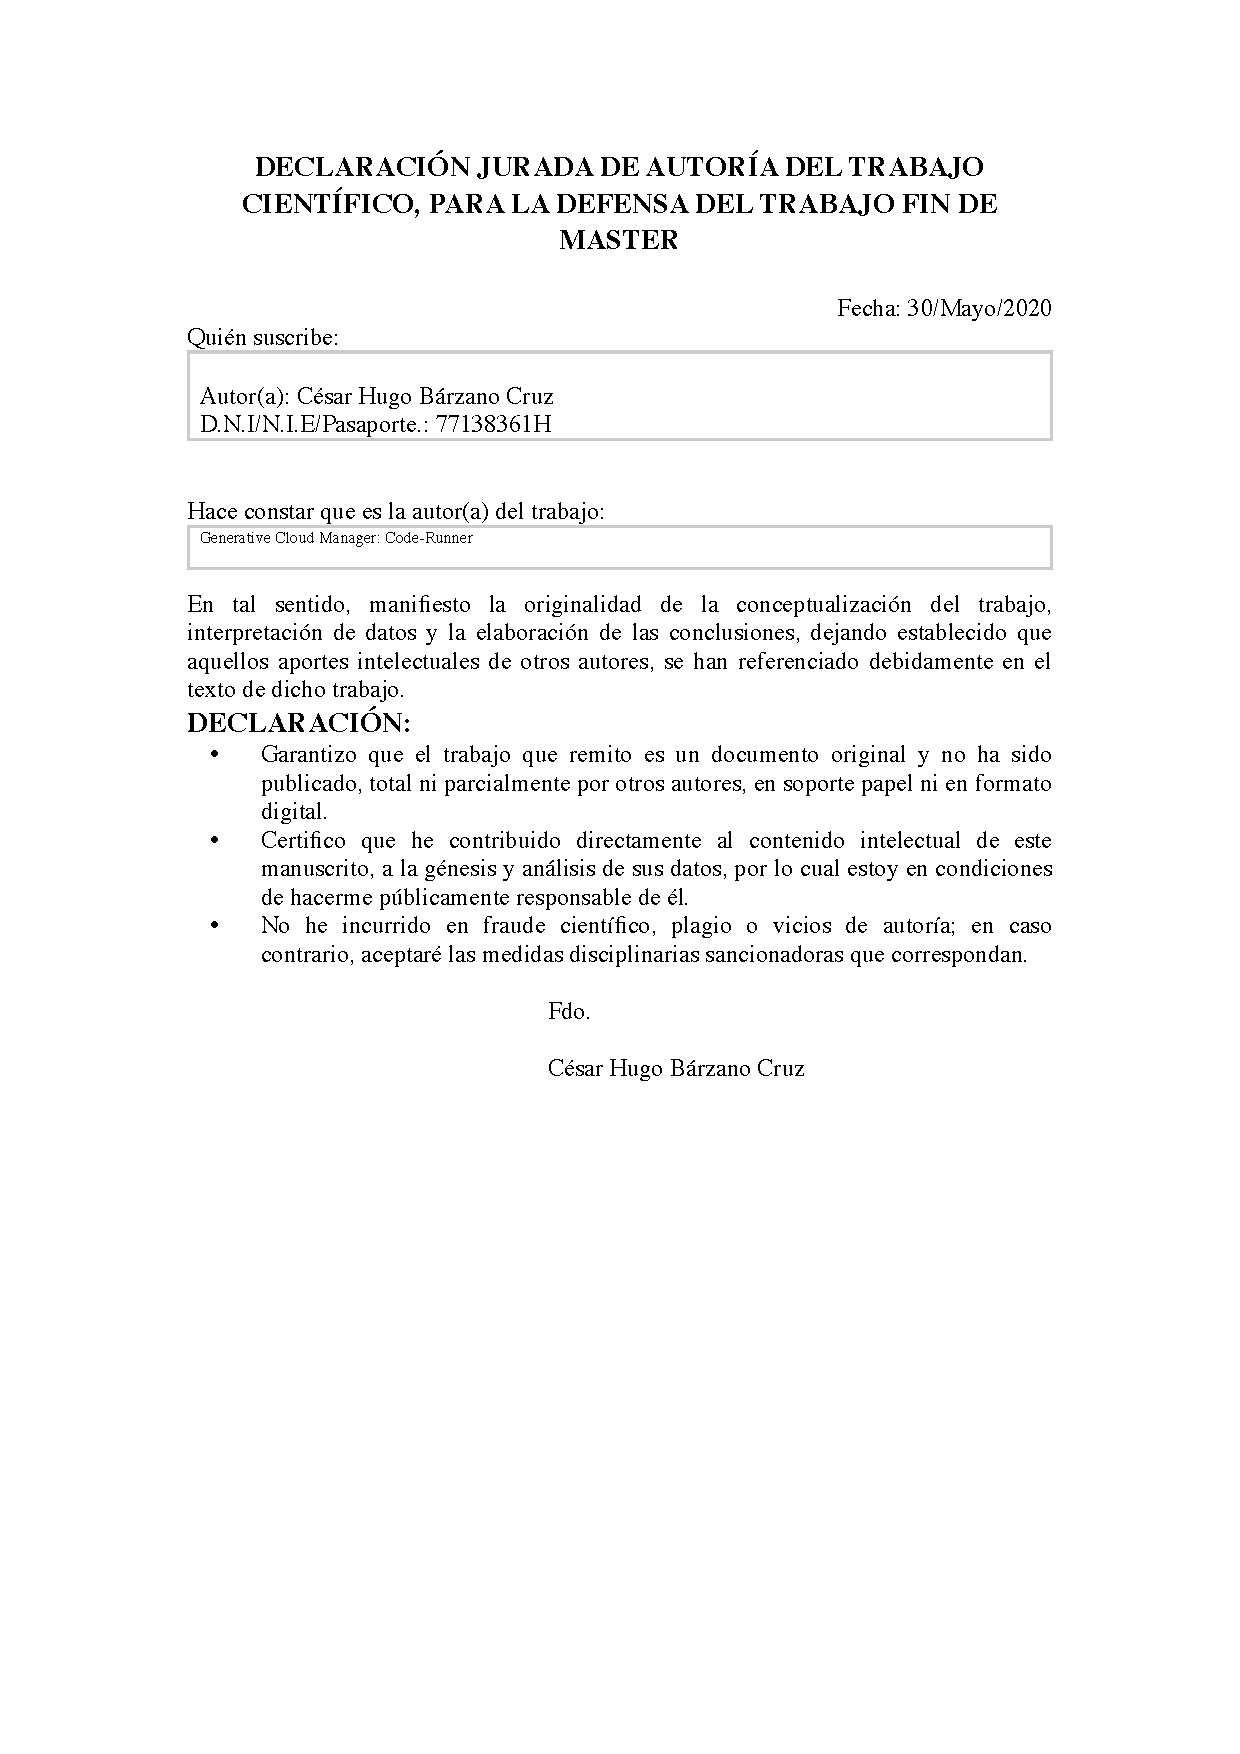
\includepdf{declara}

\afterpage{\null\newpage}
\newpage



\end{minipage}

%\vspace{2.5cm}
%\noindent\hspace*{\centeroffset}\begin{minipage}{\textwidth}
%\setlength{\centeroffset}{-0.5\oddsidemargin}
%\addtolength{\centeroffset}{0.5\evensidemargin}
%\thispagestyle{empty}
%\centering
%{\Huge\bfseries DECLARACIÓN JURADA DE AUTORÍA DEL TRABAJO CIENTÍFICO, PARA LA DEFENSA DEL TRABAJO FIN DE MASTER
%\\}
%\textbf{Quien suscribe:}\\[4.5ex]
%\textbf{Autor(a)}\\ {César Hugo Bárzano Cruz}\\[2.5ex]
%\textbf{D.N.I/N.I.E/Pasaporte.:}\\ {77138361H}\\[2.5ex]
%
%\textbf{Hace constar que es la autor(a) del trabajo:}\\ {Generative Cloud Manager: Code-Runner}\\[2.5ex]
%\textbf{Fecha}\\ {30 de Mayo de 2020}\\[2.5ex]
%
%En tal sentido, manifiesto la originalidad de la conceptualización del trabajo, interpretación de datos y la elaboración de las conclusiones, dejando establecido que aquellos aportes intelectuales de otros autores, se han referenciado debidamente en el texto de dicho trabajo.
%
%\textbf{DECLARACIÓN:}
%
%\begin{itemize}
%\item Garantizo que el trabajo que remito es un documento original y no ha sido publicado, total ni parcialmente por otros autores, en soporte papel ni en formato digital.
%\item Certifico que he contribuido directamente al contenido intelectual de este manuscrito, a la génesis y análisis de sus datos, por lo cual estoy en condiciones de hacerme públicamente responsable de él.
%\item No he incurrido en fraude científico, plagio o vicios de autoría; en caso contrario, aceptaré las medidas disciplinarias sancionadoras que correspondan
%\end{itemize}
%
%\textbf{Fdo.}\\ { César Hugo Bárzano Cruz}\\[2.5ex]
%
%\afterpage{\null\newpage}
%\newpage
%\end{minipage}
